\chapter{Evaluation Circuit}
\label{sec:EvaluationCircuit}

\section{Leiterplattenlayout mit Eagle (Viviane Bremer)}
\label{sec:eagle}

Nachdem die Auswerteschaltung in den vorigen Kapiteln dimensioniert worden ist, wird nun die Platine designt. Mit der Software Eagle wird zun�chst wieder der Schaltplan erstellt. Dieser ist in Abbildung \ref{fig:Eagle} dargestellt. Die Schaltung von zuvor wurde hier mit einem Sensoranschluss, einem Platinenstecker zur Spannungsversorgung, einer Spannungsstabilisierung f�r den IC, zwei Jumpern zum Wechseln der Br�ckenspannung und vier Platinensteckern zum Anschluss von Messger�ten erweitert. 

\begin{figure}
	\centering
	\rotatebox{90}{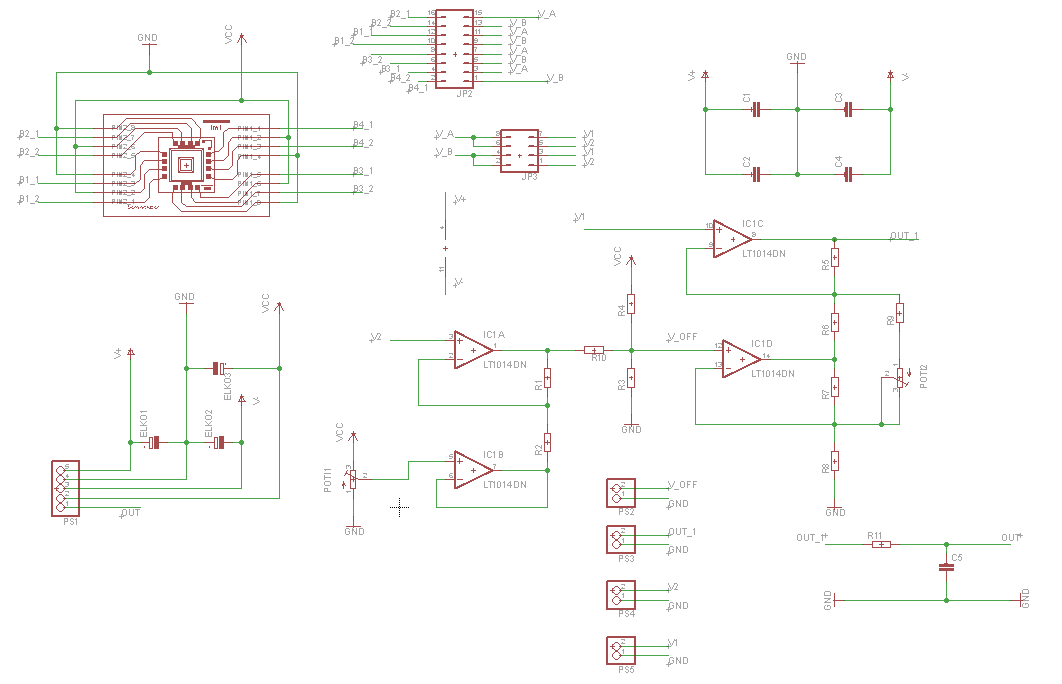
\includegraphics[width=\textheight]{figures/Auswerteelektronik.PNG}}
	\caption{Eagle-Schaltplan der Auswerteelektronik}\label{fig:Eagle}
\end{figure}

Mit dem fertigen Schaltplan kann schlie�lich die Platine erzeugt werden. Hierf�r  wird zun�chst die Gr��e \unit[3150x1969]{mil} f�r die Platine eingestellt. Danach m�ssen alle Bauteile sinnvoll platziert und verbunden werden. Eine m�gliche L�sung ist in Abbildung \ref{fig:EagleBoard} zu sehen.

\begin{figure}
	\centering
	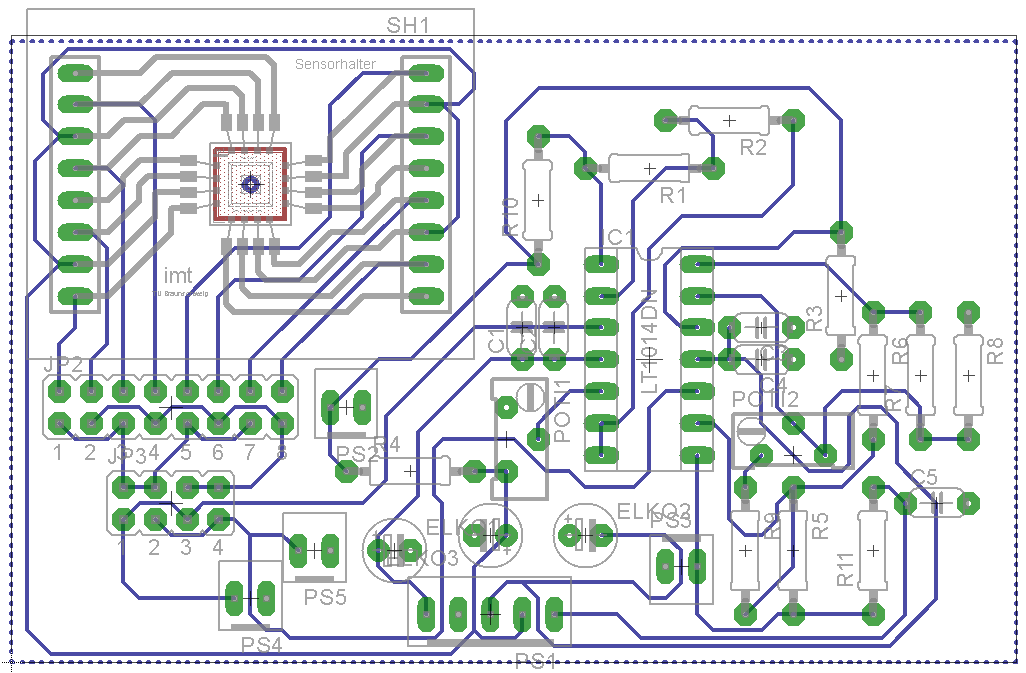
\includegraphics[width=\textwidth]{figures/Auswerteelektronik_Board.PNG}
	\caption{Platinenlayout der Auswerteelektronik in Eagle mit ausgeblendeter Massefl�che}\label{fig:EagleBoard}
\end{figure}